\documentclass[14pt]{article}
\usepackage{url}
\usepackage{hyperref}
\usepackage{amsmath}
\usepackage{mathtools}
\usepackage{extsizes}
\usepackage{titling}
\usepackage{siunitx}
\usepackage{graphicx}
\usepackage[shortlabels]{enumitem}
\usepackage[margin=0.75in]{geometry}


\newcommand{\bd}{\textbf}

\setlength{\droptitle}{-5em} 

\title{Written Homework 1}
\author{Mitchell Meier}
\date{\today}

\begin{document}

\maketitle

\begin{enumerate}

\item

\begin{enumerate}[(a)]

\item
\begin{itemize}
\item \bd{Name of individual} is qualitative nominal 
\item \bd{Systolic blood pressure} is quantitative discrete (at least in this data set) 
\item \bd{Age in years} is qualitative discrete 
\item \bd{Weight in pounds} is qualitative discrete (at least in this data set where it is rounded, is usually a qualitative ordinal value) 
\item \bd{Smoking/Nonsmoking} is qualitative nominal 
\item \bd{Level of physical activity} is qualitative ordinal in this study (goes from bottom to top poor, normal, good, excellent) 
\end{itemize}

\item

\subsection*{Analysis 1}

\subsection*{Analysis 2}


\begin{figure}[h]
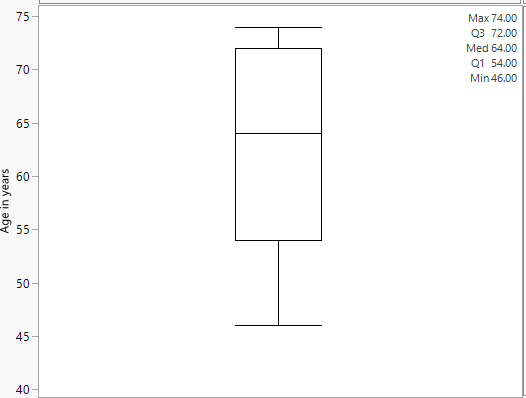
\includegraphics[scale=0.75]{hw1Pics/ageboxplot.PNG}
\centering
\end{figure}

\begin{figure}[h]
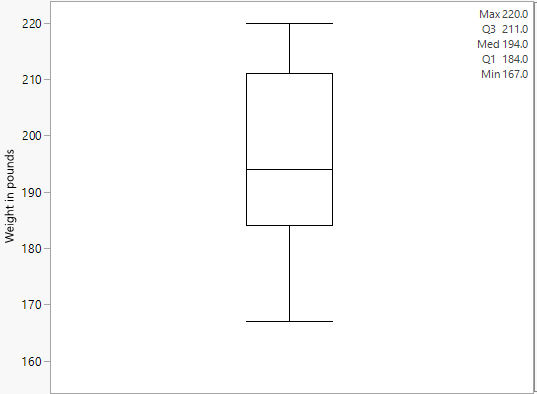
\includegraphics[scale=0.75]{hw1Pics/weightboxplot.PNG}
\centering
\end{figure}

\begin{figure}[h]
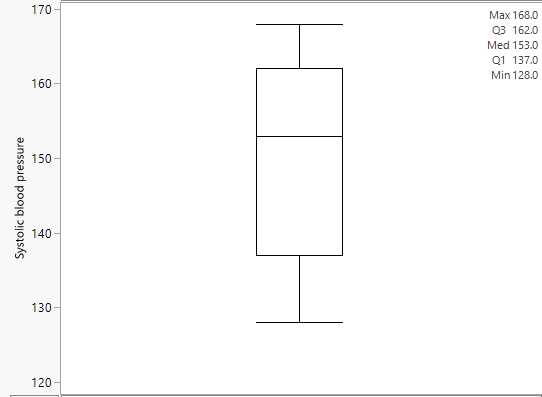
\includegraphics[scale=0.75]{hw1Pics/bpboxplot.PNG}
\centering
\end{figure}


\end{enumerate}

\item
\bd{I - Individual} 

The individual in this survey is the student. The surveryors are analyzing a trait that the S\&T student has \\

\bd{V - Variable} 

The variable in this survey is the opinion on online classes. The student's preference on fully online classes is the piece of information the surveyors are recording \\

\bd{P - Population} 

I believe the population is the S\&T community, since the prompt mentions that the survey includes the entire S\&T community. Even though this survey is only focusing on students, it most likely is just a part of a study focused on the S\&T community as a whole. If it is not, then the population would just be students \\

\bd{P - Parameter} 

The parameter for this survey is the proportion of students who prefer fully online classes. Meaning they want to know that a student either prefers or does not prefer fully online classes, then keep a running tally of each to compare them \\

\bd{S - Sample} 

The sample, or subset of the population, that the surveyors chose was 100 students from S\&T \\

\bd{S - Statistic} 

The statistic for this survey would be the proportion of S\&T students (out of the 100 in the sample) who prefer fully online classes \\



\item

\begin{enumerate}[(a)]

\item
The \bd{response variable} is the observed battery life that results from the battery being subjected to a certain material type and temperature 

\item 
The \bd{factors} are material type and temperature. The \bd{factor levels} for material type are listed as material 1, 2, and 3, and the levels for the temerature are 15\si{\degree}F, 70\si{\degree}F, and 125\si{\degree}F 

\item
The number of \bd{treatment combinations}, or different combination of factors is $3^2 = 9$, since there are 3 levels per factor, and two total factors. The \bd{treatment conditions} are: \\

MType 1 and 15\si{\degree}F, MType 1 and 70\si{\degree}F, MType 1 and 125\si{\degree}F \\
MType 2 and 15\si{\degree}F, MType 2 and 70\si{\degree}F, MType 2 and 125\si{\degree}F \\
MType 3 and 15\si{\degree}F, MType 3 and 70\si{\degree}F, MType 3 and 125\si{\degree}F \\

\item
The number of \bd{replications} total is the number of treatment combinations (9) times the number of replications each treatment combination recieves (4)
\[
9 \times 4 = 36
\]
which gives us 36 total replications 

\end{enumerate}

\end{enumerate}

\end{document}